\documentclass[aspectratio=169]{../latex_main/tntbeamer}  % you can pass all options of the beamer class, e.g., 'handout' or 'aspectratio=43'
\usepackage{dsfont}
\usepackage{bm}
\usepackage[english]{babel}
\usepackage[T1]{fontenc}
%\usepackage[utf8]{inputenc}
\usepackage{graphicx}
\graphicspath{ {./figures/} }
\usepackage{algorithm}
\usepackage[ruled,vlined,algo2e,linesnumbered]{algorithm2e}
\usepackage{hyperref}
\usepackage{booktabs}
\usepackage{mathtools}

\usepackage{amsmath,amssymb}

\DeclareMathOperator*{\argmax}{arg\,max}
\DeclareMathOperator*{\argmin}{arg\,min}

\usepackage{amsbsy}
\newcommand{\vect}[1]{\bm{#1}}
%\newcommand{\vect}[1]{\boldsymbol{#1}}

\usepackage{pgfplots}
\pgfplotsset{compat=1.16}
\usepackage{tikz}
\usetikzlibrary{trees} 
\usetikzlibrary{shapes.geometric}
\usetikzlibrary{positioning,shapes,shadows,arrows,calc,mindmap}
\usetikzlibrary{positioning,fadings,through}
\usetikzlibrary{decorations.pathreplacing}
\usetikzlibrary{intersections}
\pgfdeclarelayer{background}
\pgfdeclarelayer{foreground}
\pgfsetlayers{background,main,foreground}
\tikzstyle{activity}=[rectangle, draw=black, rounded corners, text centered, text width=8em]
\tikzstyle{data}=[rectangle, draw=black, text centered, text width=8em]
\tikzstyle{myarrow}=[->, thick, draw=black]

% Define the layers to draw the diagram
\pgfdeclarelayer{background}
\pgfdeclarelayer{foreground}
\pgfsetlayers{background,main,foreground}

% Requires XeLaTeX or LuaLaTeX
%\usepackage{unicode-math}

\usepackage{fontspec}
%\setsansfont{Arial}
\setsansfont{RotisSansSerifStd}[ 
Path=../latex_main/fonts/,
Extension = .otf,
UprightFont = *-Regular,  % or *-Light
BoldFont = *-ExtraBold,  % or *-Bold
ItalicFont = *-Italic
]
\setmonofont{Cascadia Mono}[
Scale=0.8
]

\renewcommand{\ttdefault}{Cascadia Mono}

% scale factor adapted; mathrm font added (Benjamin Spitschan @TNT, 2021-06-01)
%\setmathfont[Scale=1.05]{Libertinus Math}
%\setmathrm[Scale=1.05]{Libertinus Math}

% other available math fonts are (not exhaustive)
% Latin Modern Math
% XITS Math
% Libertinus Math
% Asana Math
% Fira Math
% TeX Gyre Pagella Math
% TeX Gyre Bonum Math
% TeX Gyre Schola Math
% TeX Gyre Termes Math

% Literature References
\newcommand{\lit}[2]{\href{#2}{\footnotesize\color{black!60}[#1]}}

%%% Beamer Customization
%----------------------------------------------------------------------
% (Don't) Show sections in frame header. Options: 'sections', 'sections light', empty
\setbeamertemplate{headline}{empty}

% Add header logo for normal frames
\setheaderimage{
	% 
\includegraphics[height=\logoheight]{figures/TNT_darkv4.pdf}
	
\includegraphics[height=\logoheight]{../latex_main/figures/Leibniz-AI-Academy_Logo}
	% 
\includegraphics[height=\logoheight]{figures/logo_tntluh.pdf}
}

% Header logo for title page
\settitleheaderimage{
	% 
\includegraphics[height=\logoheight]{figures/TNT_darkv4.pdf}
	
\includegraphics[height=\logoheight]{../latex_main/figures/Leibniz-AI-Academy_Logo}
	% 
\includegraphics[height=\logoheight]{figures/logo_tntluh.pdf}
}

% Title page: tntdefault 
\setbeamertemplate{title page}[tntdefault]  % or luhstyle
% Add optional title image here
%\addtitlepageimagedefault{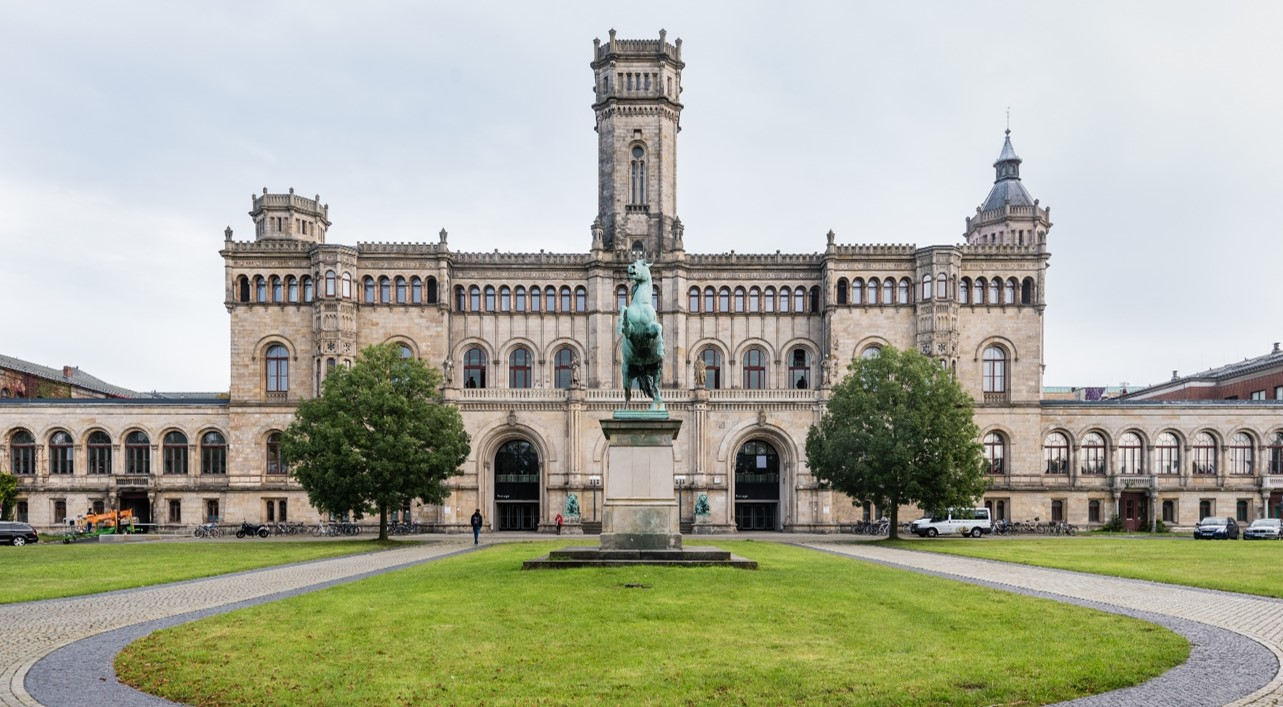
\includegraphics[width=0.65\textwidth]{figures/luh_default_presentation_title_image.jpg}}

% Title page: luhstyle
% \setbeamertemplate{title page}[luhstyle]
% % Add optional title image here
% \addtitlepageimage{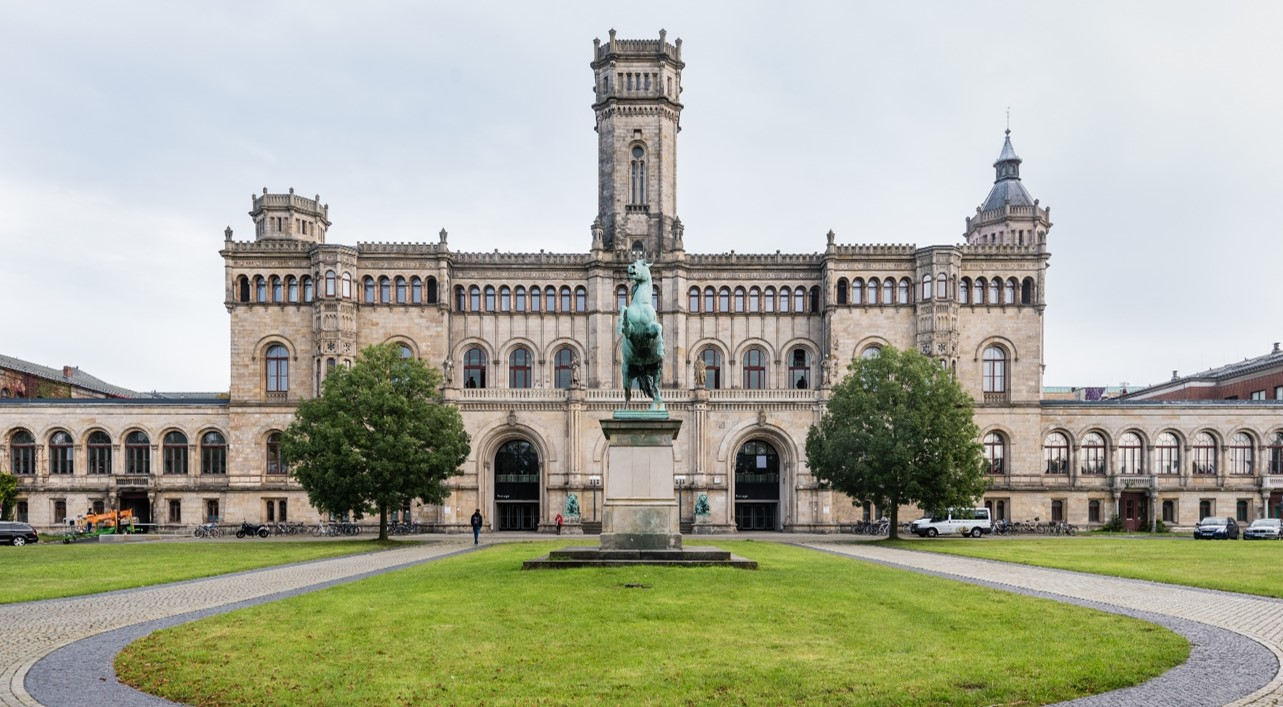
\includegraphics[width=0.75\textwidth]{figures/luh_default_presentation_title_image.jpg}}

\author[Abedjan \& Lindauer]{Ziawasch Abedjan \& \underline{Marius Lindauer}\\[1em]
	%
\includegraphics[height=\logoheight]{../latex_main/figures/luh_logo_rgb_0_80_155.pdf}\qquad
	
\includegraphics[height=\logoheight]{../latex_main/figures/DBIS_Kurzlogo.png}\qquad
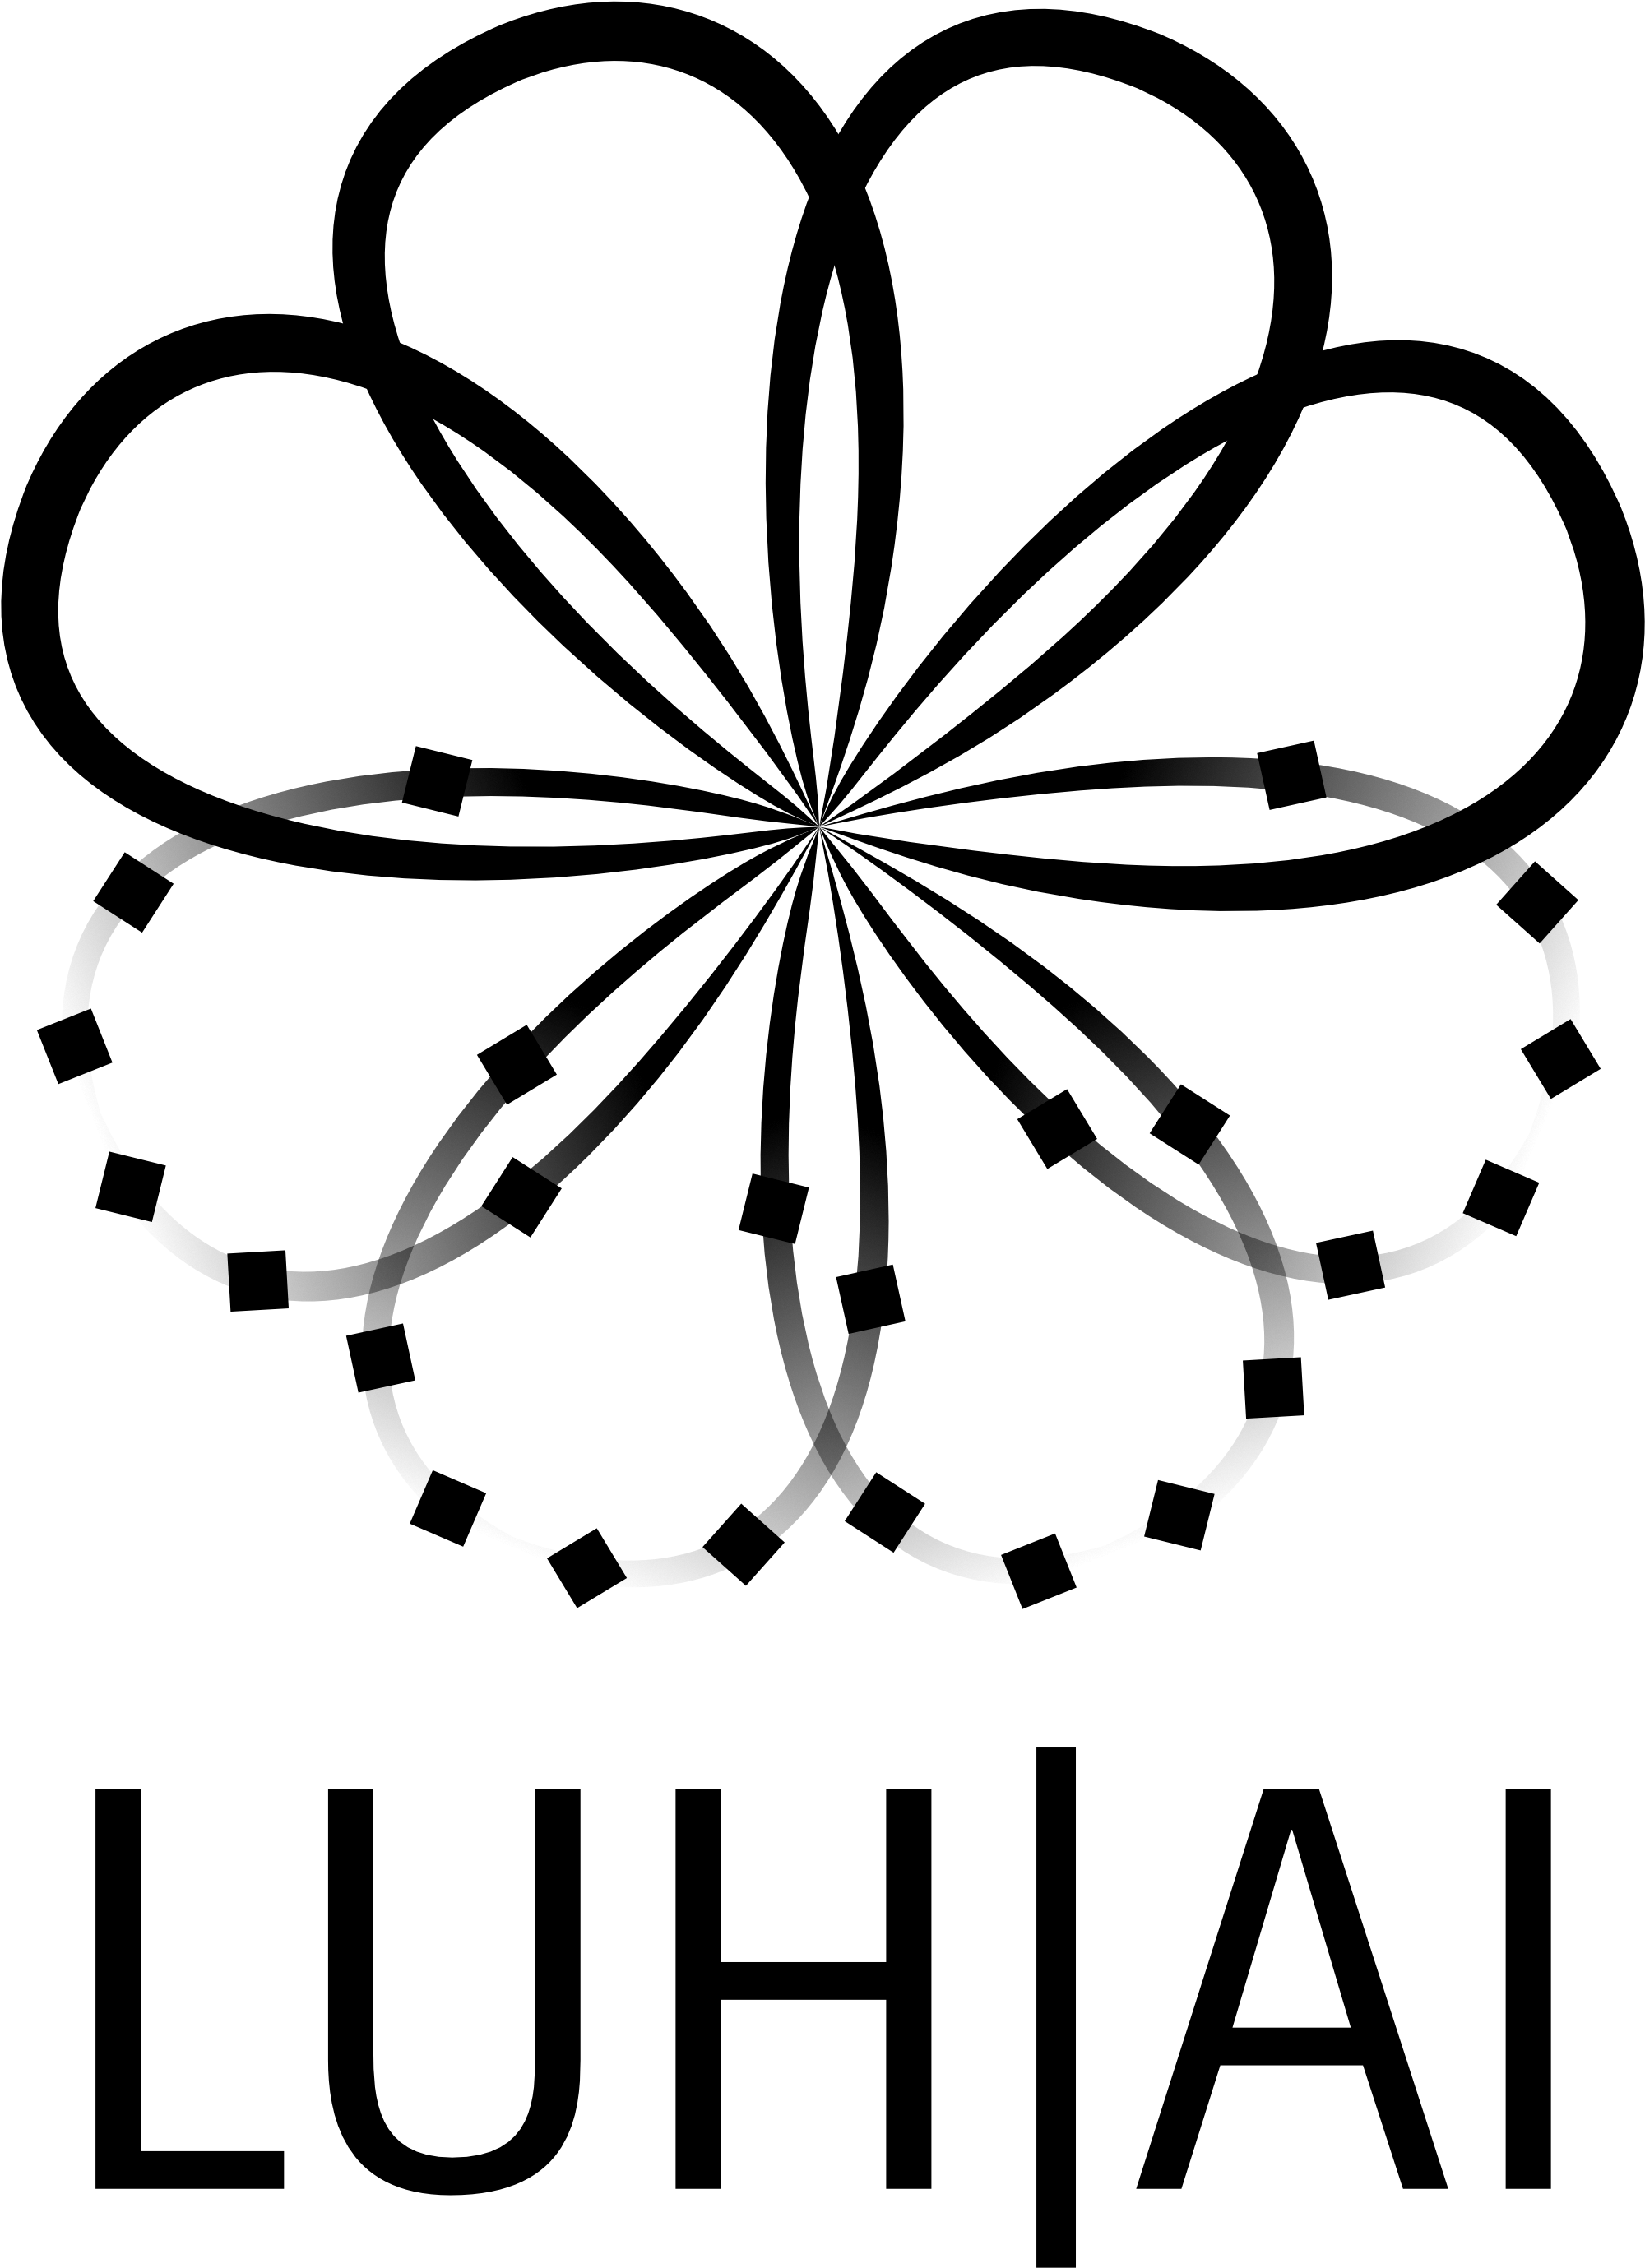
\includegraphics[height=\logoheight]{../latex_main/figures/logo_short_highres_black}\qquad

\includegraphics[height=\logoheight]{../latex_main/figures/Leibniz-AI-Academy_Logo}\qquad
%
\includegraphics[height=\logoheight]{../latex_main/figures/L3S.jpg}	
}
\date{\hspace{0.5em} {
\includegraphics[height=1.5em]{../latex_main/figures/Cc-by-nc-sa_icon.svg.png}}; extension of \href{https://ds100.org/fa21/}{[DS100]}
}


%%% Custom Packages
%----------------------------------------------------------------------
% Create dummy content
\usepackage{blindtext}

% Adds a frame with the current page layout. Just call \layout inside of a frame.
\usepackage{layout}


%%% Macros
%\renewcommand{\vec}[1]{\mathbf{#1}}
% \usepackage{bm}
%\let\vecb\bm

\title[Standardizing Data]{DS: Data Cleaning}
\subtitle{Standardizing Data}

\graphicspath{ {./figure/} }
%\institute{}


\begin{document}
	
	\maketitle

\begin{frame}[c]{Goal 1: Joining Tables with Mismatched Labels}

\centering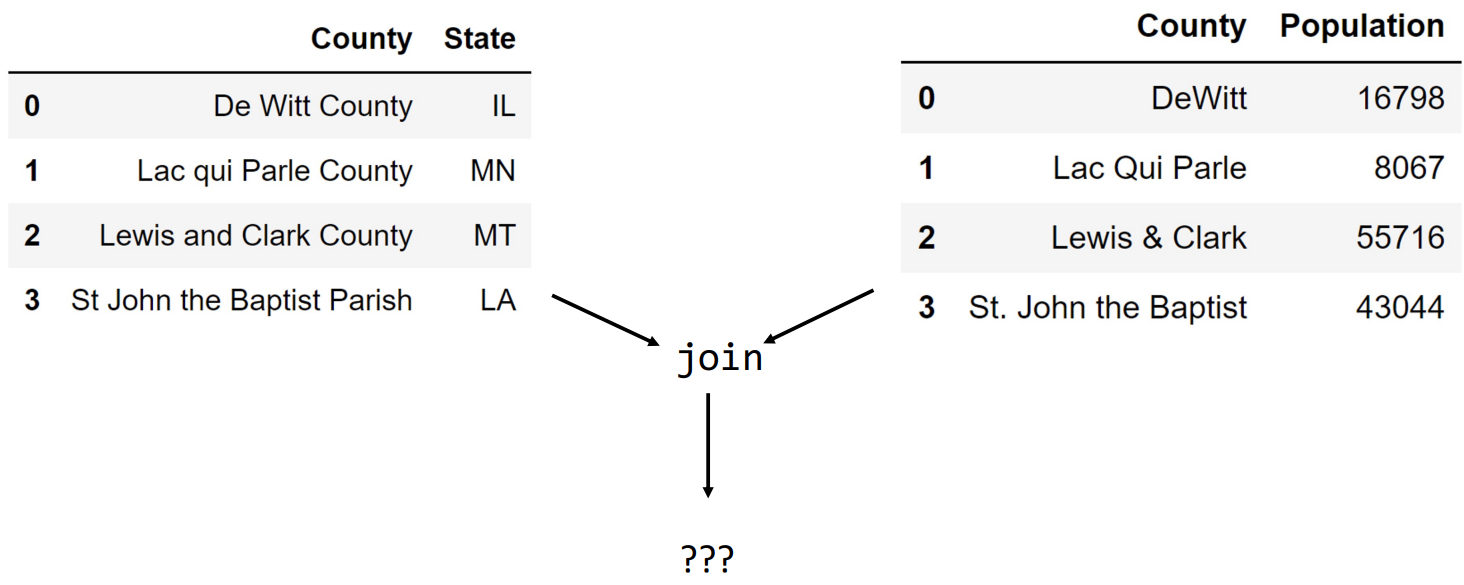
\includegraphics[width=0.7\textwidth]{figure/bild23_join}

\begin{itemize}
    \item To join tables, unify the county names
    \item \textbf{Unify/Standardize}: Convert data that has more than one possible representation into a standard form
\end{itemize}

\end{frame}


\begin{frame}[c]{Unifying County Names}

\centering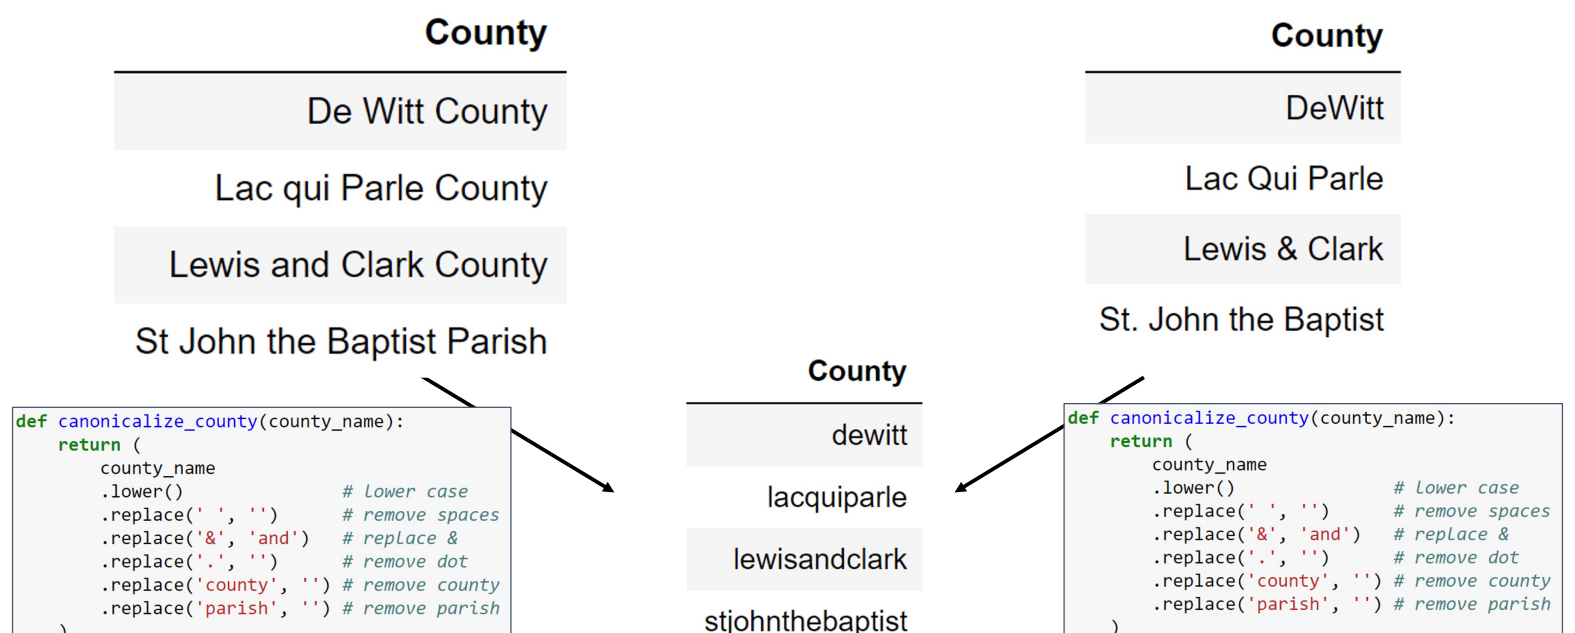
\includegraphics[width=1.0\textwidth]{figure/bild23_join2}

\end{frame}

\begin{frame}[c]{Unifying Strings}

\begin{itemize}
    \item Replace each string with a unique representation
    \begin{itemize}
        \item Feels hacky, but messy problems often require messy solutions
        \item Can be done slightly better but requires maintenance
    \end{itemize}
    \item \textbf{Tools used:}
    \begin{itemize}
        \item Replacement: \texttt{str.replace(‘\&’, ‘and’)}
        \item Deletion: \texttt{str.replace(‘ ’, ‘’)}
        \item Transformation: \texttt{str.lower()}
    \end{itemize}
\end{itemize}

\end{frame}

\begin{frame}[c]{Duplicate Detection}

\begin{itemize}
    \item Duplicate detection is the discovery of multiple representations of the same real-world object
    \item \textbf{Problem 1}: Representations are not identical (fuzzy duplicates)
    \begin{itemize}
        \item Solution: Similarity measures 
        \begin{itemize}
            \item value- and record-comparisons
            \item domain-dependent or domain-independent
        \end{itemize}
    \end{itemize}
    \item \textbf{Problem 2}: Data sets are large (quadratic complexity in comparing every pair of records)
    \begin{itemize}
        \item Solution: Algorithms (e.g., avoid comparisons by partitioning)
    \end{itemize}
\end{itemize}

\end{frame}

\begin{frame}[c]{Duplicate Detection: Example Process}

\centering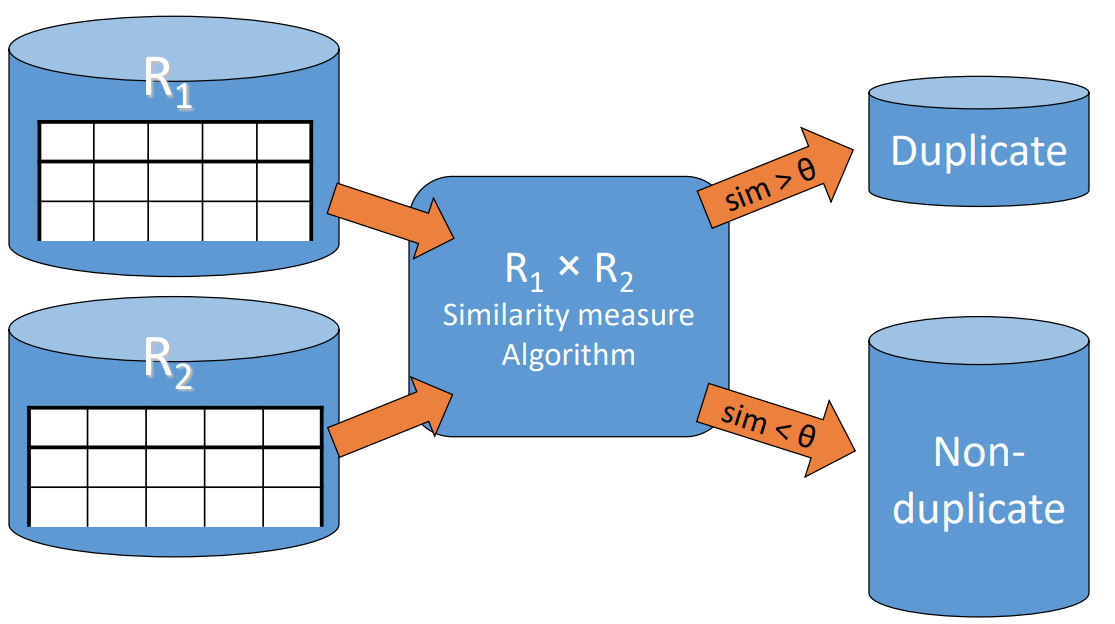
\includegraphics[width=0.7\textwidth]{figure/bild25_duplicates}

\begin{itemize}
    \item Process showing record comparisons with similarity measure and classification into duplicate or non-duplicate
\end{itemize}

\end{frame}

\begin{frame}[c]{Similarity Measures}

\begin{columns}

    \column{0.5\textwidth}

    \begin{itemize}
        \item \textbf{Edit-Distance:} Minimal number of edit operations to change one word into another
        \begin{itemize}
            \item Example: Naumann $\rightarrow$ Neumann (1 edit), Naumann $\rightarrow$ Müller (7 edits)
        \end{itemize}
        \item \textbf{Jaro / Jaro-Winkler:} Common letters within half string length; handles transposed letters
        \item \textbf{Soundex:} 4-letter code for each word (e.g., SOUNDEX('Farwick') = F620)
        \begin{itemize}
            \item Also: Kölner Phonetik for German terms
        \end{itemize}
    \end{itemize}


    \column{0.5\textwidth}

        \centering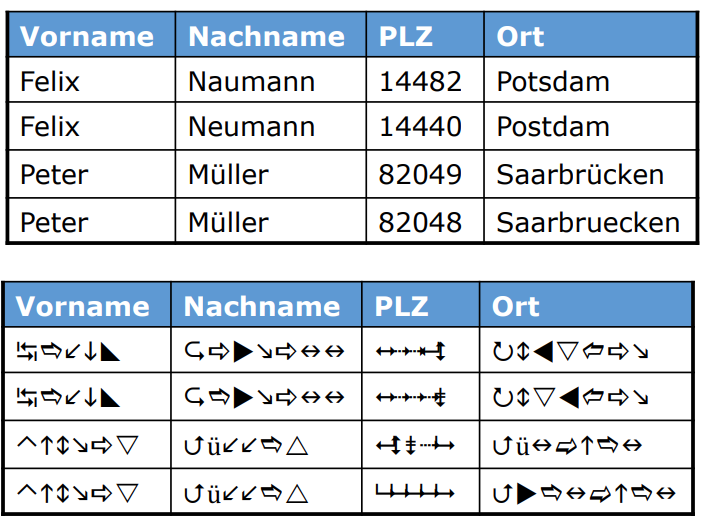
\includegraphics[width=0.8\textwidth]{figure/bild26_similarity}

\end{columns}

\end{frame}


\begin{frame}[c]{Number of Comparisons}

\begin{itemize}
    \item \textbf{Problem}: Too many comparisons!
    \begin{itemize}
        \item Example: 10,000 customers $\rightarrow$ 49,995,000 comparisons 
        \item There are ($(n^2 -n) /2 $) since you don't need to compare on the diagonal and only half of the matrix since the symmetries are symmetric
    \end{itemize}
    \item Each comparison is computationally expensive
    \item \textbf{Idea}: Avoid unnecessary comparisons by:
    \begin{itemize}
        \item Filtering out individual records
        \item Partitioning records and comparing only within each partition
    \end{itemize}
\end{itemize}

\end{frame}

\begin{frame}[c]{Partitioning / Blocking}

\begin{columns}

    \column{0.5\textwidth}

        \begin{itemize}
            \item \textbf{Partitioning:} Divide records horizontally, compare only within a partition
            \begin{itemize}
                \item Example: Partition by first two zip-digits
                \begin{itemize}
                    \item Approx. 100 partitions in Germany, 100 customers per partition $\to$ 495,000 comparisons
                \end{itemize}
                \item Partition by first letter of surname, etc.
            \end{itemize}
            \item \textbf{Idea:} Apply multiple partitioning criteria, then apply transitive closure on duplicates
            \begin{itemize}
                \item Balancing speed with accuracy
            \end{itemize}
        \end{itemize}

    \column{0.5\textwidth}

        \centering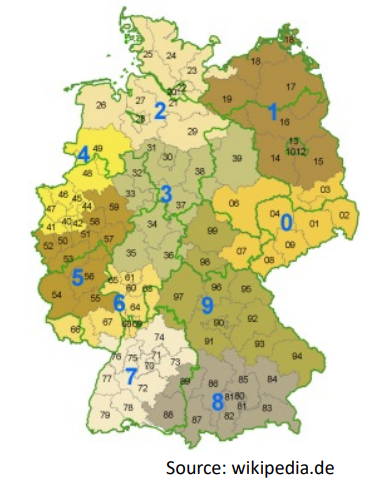
\includegraphics[width=0.7\textwidth]{figure/bild27_part}
    
\end{columns}


\end{frame}


\begin{frame}[c]{Summary: Data Preparation}

\begin{itemize}
    \item \textbf{Examine data and metadata:}
    \begin{itemize}
        \item Assess date, size, organization, and structure
    \end{itemize}
    \item Examine each field/attribute individually
    \item Examine pairs of related dimensions
    \item \textbf{Stratify earlier analysis:} Break down by relevant categories (e.g., grades by major)
    \item \textbf{Along the way:}
    \begin{itemize}
        \item Visualize and summarize data
        \item Validate assumptions about data and collection process
        \item Identify and address anomalies
        \item Apply data transformations and corrections
        \item Record every step and rationale
    \end{itemize}
\end{itemize}

\end{frame}

\end{document}